\documentclass[12pt, letterpaper]{article}

% --- PACKAGES ---
\usepackage[utf8]{inputenc}
\usepackage{amsmath}
\usepackage{graphicx}
\usepackage[margin=1in]{geometry}
\usepackage{fancyhdr}
\usepackage{times}
\usepackage{hyperref}
\usepackage{float}
\usepackage{caption}
\usepackage{subcaption}
\usepackage{booktabs}
\usepackage{setspace}

% --- DOCUMENT INFORMATION ---
\title{Optimizing Energy Generation: Leveraging Electric Vehicle Battery Storage for Grid Stabilization}
\author{Grayson Adams \\ \texttt{gtadams@mit.edu} \and
        Shane Pornprinya \\ \texttt{shaneppy@mit.edu} \and
        Becca Sholler \\ \texttt{rsholler@mit.edu}}
\date{August 6, 2025}

% --- HEADER & FOOTER ---
\pagestyle{fancy}
\fancyhf{}
\lhead{15.066 Final Project}
\rhead{Group 5A}
\cfoot{\thepage}

\begin{document}

\maketitle
\thispagestyle{empty}

% --- TABLE OF CONTENTS ---
\onehalfspacing
\tableofcontents

\newpage

% --- MAIN BODY ---
\section{Introduction}
\noindent Electrical utility providers face the complex challenge of balancing energy generation costs, greenhouse gas emissions, and fluctuating consumer demand. This landscape is further complicated by the rising energy needs from electric vehicle (EV) adoption and AI data centers, alongside increasingly stringent CO2 emissions targets. This report explores a novel solution: utilizing the growing fleet of electric vehicles as a distributed battery bank to optimize power generation. We develop and solve a linear programming optimization model to determine the least-cost energy generation mix for the state of California, both with and without the use of Vehicle-to-Grid (V2G) technology. Our findings indicate that integrating EVs for grid storage can lead to significant daily cost savings of approximately \$1.4 million, primarily by enabling greater use of low-cost renewables and reducing reliance on expensive and higher-emission peaker plants. The analysis also demonstrates the sensitivity of these savings to the installed capacity of renewable sources, particularly solar. This project highlights the potential of V2G as a critical tool for creating a more cost-effective, resilient, and sustainable energy grid.

The electrical utility sector is at a critical juncture. The traditional model of centralized power generation is being challenged by a confluence of powerful forces. On one hand, total energy demand is on a sharp upward trajectory, fueled by the widespread adoption of electric vehicles (EVs) and the exponential growth of energy-intensive data centers required for artificial intelligence (AI). On the other hand, there is immense pressure to decarbonize the energy sector to mitigate the impacts of climate change, leading to aggressive CO2 emissions reduction targets. Compounding these challenges is the persistent political and social pressure to keep electricity prices affordable for consumers. This creates a complex, multi-variable problem for utility providers who must continuously balance three competing priorities:
\begin{itemize}
    \item \textbf{Cost:} Minimizing the operational cost of energy generation to ensure affordability.
    \item \textbf{Emissions:} Reducing the environmental impact, specifically greenhouse gas emissions.
    \item \textbf{Demand:} Reliably meeting the ever-changing energy needs of consumers.
\end{itemize}

This project investigates a promising pathway to address this trilemma: leveraging the rapidly expanding fleet of electric vehicles as a distributed energy storage system. The core question we seek to answer is: \textbf{How can electrical utilities make effective use of the aggregated battery capacity of electric vehicles in their service area to improve operational performance, reduce costs, and lower emissions?} This concept, known as Vehicle-to-Grid (V2G), proposes that EVs can not only draw energy from the grid to charge but also inject energy back into the grid when needed. This turns millions of cars into a massive, decentralized battery bank that can help stabilize the grid, absorb excess renewable energy, and provide power during peak demand hours.

\section{Data and Methodology}

To build our optimization model, we gathered data from several authoritative sources such as EIA and NREL, and employed predictive modeling to estimate key parameters. The analysis is framed from the perspective of a single utility provider servicing the entire state of California.

\subsection{Data Sources}
Our model relies on the following key data inputs:
\begin{itemize}
    \item \textbf{Levelized Cost of Energy (LCOE):} The total lifecycle cost to build and operate a power plant, expressed in \$/MWh for each fuel source (e.g., natural gas, solar, wind). This data was sourced from the U.S. Energy Information Administration (EIA).
    \item \textbf{CO2 Emissions Factors:} The lifecycle greenhouse gas emissions associated with each fuel source, measured in metric tons of CO2 per MWh. This data was also provided by the EIA.
    \item \textbf{Installed Generation Capacity:} The maximum power output for each fuel type currently available within California.
    \item \textbf{Hourly Demand Curve:} A representative 24-hour profile of electricity demand for the state of California.
    \item \textbf{Electric Vehicle Fleet Data Prediction:} To estimate the total available battery storage capacity, produced by a predictive model that projects EV fleet size based on American Communities Survey 2023 US Census data.
    \item \textbf{Daily Generation Time-Series:} To forecast daily generation capacities of fast-growing renewable energy sources to perform sensitivity analysis.
\end{itemize}

\subsubsection{Imputation}
The CAISO provided daily and weekly generation capacity and load data through their OASIS API. However, the data for solar, geothermal, natural gas, imports, other, and load are missing 0.04\% of the values. To impute the data, we assigned 80\% of the data to the training set, and the remaining 20\% to the testing set. We then compute the MAPE of 3 imputation methods: mean, median, and K-Nearest Neighbor. Because the K-Nearest Neighbor algorithm with 3 neighbors resulted in the lowest MAPE, we used the algorithm to impute missing solar data. 
\begin{table}[H]
\centering
\caption{Table comparing MAPE of mean, median and K-Nearest Neighbor imputation methods}
\label{tab:mape_solar}
\begin{tabular}{@{}lcc@{}}
\toprule
\textbf{Method} & \textbf{MAPE}  \\ \midrule
Mean        & 41.78 \\
Median      & 40.18 \\
KNN k=3     & 14.60  \\
\bottomrule
\end{tabular}
\end{table}

\begin{figure}[h]
    \centering
    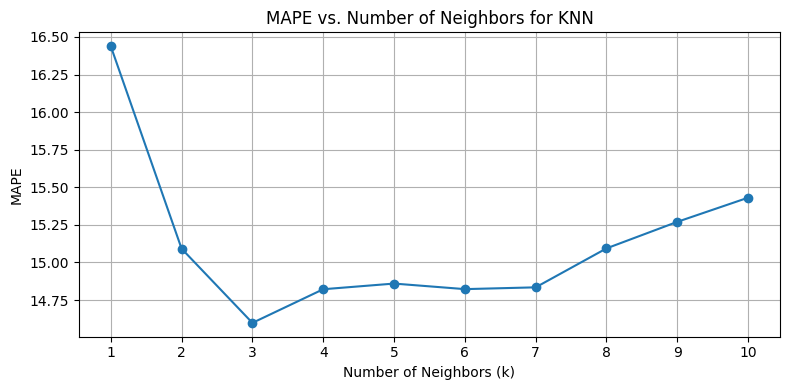
\includegraphics[width=\textwidth]{solar_knn.png}
    \caption{Plot of MAPE of each k when using the K-Nearest Neighbor algorithm to impute missing solar time-series data}
    \label{fig:solar_knn}
\end{figure}

\subsection{Predicting EV Distribution}
A critical component of this study was to estimate the number and location of EVs within the service area. Since direct data for every locality is not available, we developed a predictive model. Using EV registration data from a subset of counties as our training set, we correlated EV ownership with various demographic factors obtained from the U.S. Census Bureau (e.g., income levels, education, age distribution, political leaning).

We trained a Classification and Regression Tree (CART) model to predict EV penetration rates based on these demographic features, as well as a Random Forest. The CART model is shown to help understand the major factors that indicate the quantity of EVs per county and confirm that these align with other research and intuitive expectations. The Random Forest, while less interpretable, has similar rankings for parameter importance and a higher predictive power and was therefore used as the final model. The model achieved a strong in-sample R-squared of 0.866 and an out-of-sample R-squared of 0.752, indicating good predictive power. Figure \ref{fig:cart_tree} shows a visualization of the decision tree, and Figure \ref{fig:ca_map} shows the resulting prediction of EV distribution across California counties.

For EV predictions, the US Census data offers detailed demographic features at a county level, which are known to be strong predictors of consumer behavior like EV adoption. As discussed in further detail in "15.087 Group 5A Final Report", the training data from the model is also furnished from the respective DMVs of the states included in the model to reliably establish EV registrations per county to train on.

\begin{figure}[H]
     \centering
     \begin{subfigure}[b]{0.9\textwidth}
         \centering
         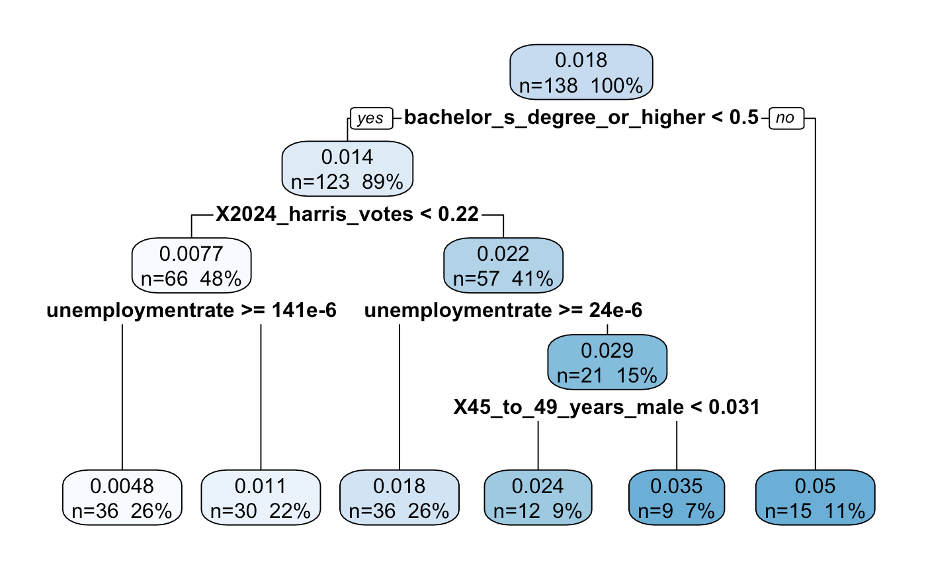
\includegraphics[width=\textwidth]{cart_model.png}
         \caption{CART decision tree for predicting EV fleet size by county with WA, OR, CA, and HI. The tree shows a prediction of higher EV counts for larger values, also shown as darker blue colors. Counties with high rates of education, left leaning political voters, and low unemployment tend to have higher EVs.}
         \label{fig:cart_tree}
     \end{subfigure}
     \vfill
     \begin{subfigure}[b]{0.9\textwidth}
         \centering
         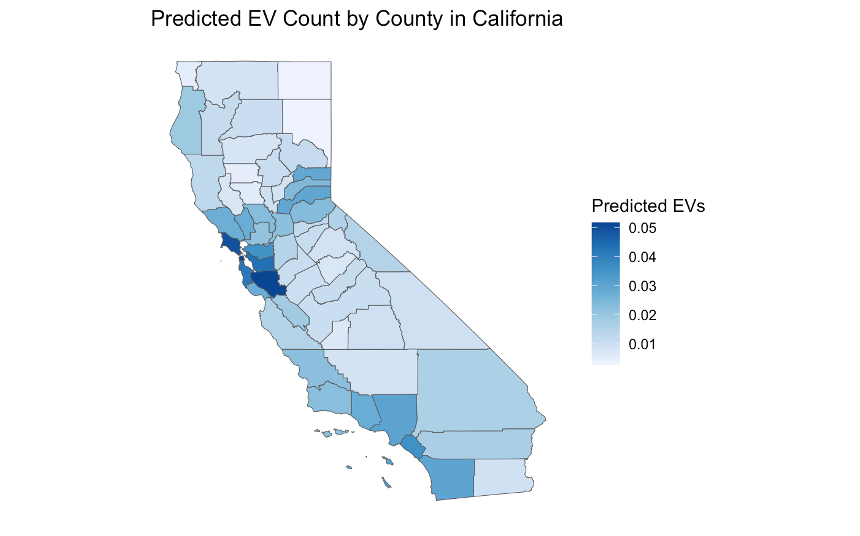
\includegraphics[width=\textwidth]{california_ev_map.png}
         \caption{Predicted EV Count by County in California geographically mapped.}
         \label{fig:ca_map}
     \end{subfigure}
        \caption{Predictive modeling results of EV distribution within the state using most current census data.}
        \label{fig:ev_prediction}
\end{figure}

\subsection{Key Assumptions}
To maintain a tractable model, we made several key assumptions:
\begin{enumerate}
    \item LCOE and CO2 emissions factors are based on national averages from the EIA.
    \item The daily demand curve represents a typical day and does not account for seasonal variations or unexpected events.
    \item The aggregated EV battery bank starts and ends each 24-hour cycle at a 50\% state of charge (SoC).
    \item Energy required for vehicle mobility is already accounted for within the total electricity demand curve.
    \item The round-trip efficiency of charging and discharging the EV batteries is 95\%.
    \item The maximum charge and discharge rate for the aggregated battery bank is C/16, meaning the full capacity can be charged or discharged over 16 hours.
    \item A generic "Other" fuel source is included to represent a mix of biogas, diesel, and imported power, characterized by high cost and medium emissions.
\end{enumerate}

\section{Optimization Model Formulation}

We formulated a linear programming model to determine the optimal hourly energy dispatch from various fuel sources to meet demand at the minimum cost, subject to operational and environmental constraints. No integer programming or nonlinearities are introduced into the optimization, and the parameters are all established as deterministic. Given that this is a fully linear program, the solution determined is the globally optimal, or at least equally optimal, among all possible solutions.

\subsection{Objective Function}
The primary objective is to minimize the total daily cost of energy generation. The cost is the sum of the energy generated from each fuel type multiplied by its respective LCOE, summed over all 24 hours of the day.

\begin{equation}
\min \sum_{i=1}^{NumFT} \sum_{t=1}^{24} Gen[i, t] \cdot C[i]
\end{equation}

Where:
\begin{itemize}
    \item $Gen[i, t]$ is the amount of energy (MWh) generated by fuel type $i$ at hour $t$.
    \item $C[i]$ is the Levelized Cost of Energy (\$/MWh) for fuel type $i$.
    \item $NumFT$ is the total number of fuel types.
\end{itemize}

\subsection{Decision Variables}
All decision variables used are continuous.
\begin{itemize}
    \item $Gen[i, t]$: Energy to generate from fuel source $i$ in hour $t$.
    \item $charge[t]$: Energy used to charge the EV battery bank in hour $t$.
    \item $discharge[t]$: Energy supplied by the EV battery bank in hour $t$.
    \item $SoC[t]$: State of Charge of the EV battery bank at the end of hour $t$.
\end{itemize}

\subsection{Constraints}
The optimization is subject to the following constraints for each hour $t \in \{1, ..., 24\}$ and each fuel type $i \in \{1, ..., NumFT\}$:

\begin{enumerate}
    \item \textbf{Demand Fulfillment:} Total generation plus energy discharged from batteries, minus energy used to charge batteries, must equal the hourly demand.
    \begin{equation}
    \sum_{i=1}^{NumFT} Gen[i, t] + discharge[t] - charge[t] = hourlyDemand[t]
    \end{equation}

    \item \textbf{Generation Capacity:} The energy generated from each fuel source cannot exceed its available capacity in that hour.
    \begin{equation}
    Gen[i, t] \leq MaxCap[i, t]
    \end{equation}

    \item \textbf{Emissions Limit:} The total CO2 emissions for the day must not exceed a predefined cap.
    \begin{equation}
    \sum_{i=1}^{NumFT} \sum_{t=1}^{24} Gen[i, t] \cdot E[i] \leq MaxCO2
    \end{equation}

    \item \textbf{Battery State of Charge (SoC) Balance:} The SoC at the end of the day must be at least the SoC at the start.
    \begin{equation}
    SoC[24] \geq SoC[1]
    \end{equation}

    \item \textbf{SoC Dynamics:} The SoC in the current hour is determined by the previous hour's SoC plus any charging and minus any discharging, adjusted for efficiency ($\eta$).
    \begin{equation}
    SoC[t] = SoC[t-1] + \eta \cdot charge[t] - discharge[t]
    \end{equation}

    \item \textbf{Battery Capacity Limits:} The SoC must remain within its operational bounds (e.g., 25\% to 100\% of total capacity).
    \begin{equation}
    0.25 \cdot BattCap \leq SoC[t] \leq BattCap
    \end{equation}

    \item \textbf{Charge/Discharge Rate:} The amount of energy charged or discharged in a single hour is limited by the maximum rate.
    \begin{gather}
    0 \leq charge[t] \leq MaxChgRate \\
    0 \leq discharge[t] \leq MaxChgRate
    \end{gather}

    \item \textbf{Rate of Capacity Change:} The capacity of natural gas, nuclear, and hydroelectric is limited.
    \begin{gather}
    Gen[i, t] - Gen[i,t-1] \leq R[i] \quad \text{(Ramp-up)} \\
    Gen[i,t-1] - Gen[i,t] \leq R[i] \quad \text{(Ramp-down)}
    \end{gather}
    
\end{enumerate}

\subsubsection{Parameters}
\begin{itemize}
    \item $C[i]$: Cost in \$/MWh per fuel type $i$
    \item $E[i]$: CO2 emissions in metric tons per MWh per fuel type $i$
    \item $NumFT$: Number of fuel types available
    \item $MaxCO2$: Maximum total CO2 emissions across all fuels in metric tons, daily
    \item $BattCap$: Aggregate EV bank capacity in MWh, calculated as sum of EVs in service area from predictive model multiplied by average battery capacity of 80 kWh
    \item $MaxChgRate$: Maximum rate at which the battery bank may charge or discharge
    \item $\eta$ : Battery bank charge efficiency
    \item $hourlyDemand[t]$: Total energy demand at time $t$
    \item $MaxCap[i,t]$: Maximum capacity of fuel source $i$ at time $t$
    \item $R[i]$: Maximum allowable ramp rate (MW/hour) for fuel source $i$
\end{itemize}

\section{Results and Analysis}

Solving the optimization model yields the optimal hourly energy dispatch strategy. We ran the model for two scenarios: a baseline case without V2G capabilities, and a second case incorporating the EV battery bank.

\subsection{Optimal Dispatch and Cost Savings}
The results demonstrate a significant financial benefit from using V2G.
\begin{itemize}
    \item \textbf{Cost without V2G:} \$27.1 million per day.
    \item \textbf{Cost with V2G:} \$25.7 million per day.
\end{itemize}
This represents a \textbf{daily savings of \$1.4 million}, or an annual savings of over \$500 million for the state.

Figure \ref{fig:dispatch_with_v2g} shows the optimal energy dispatch profile for the V2G-enabled scenario. The EV battery bank (represented by the blue line for SoC and yellow bars for discharge) plays a crucial role. During midday hours when solar generation is abundant and cheap, excess energy is used to charge the batteries (SoC increases). During the evening peak demand hours (approx. 18:00-22:00), as solar power fades, the batteries discharge this stored energy to meet demand. This "peak shaving" avoids the need to ramp up expensive and higher-emission natural gas or "Other" peaker plants.

\begin{figure}[H]
    \centering
    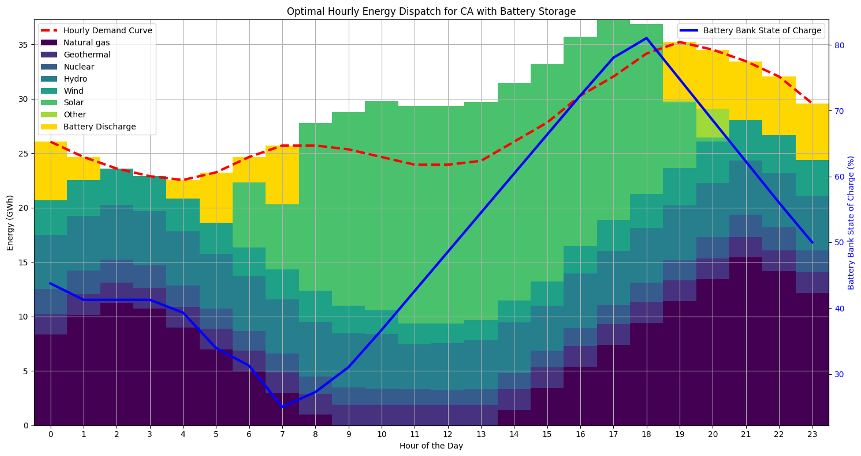
\includegraphics[width=\textwidth]{dispatch_with_v2g.png}
    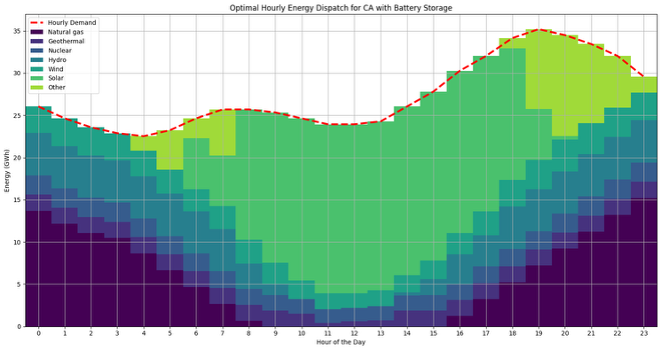
\includegraphics[width=\textwidth]{dispatch_no_v2g.png}
    \caption{Optimal Hourly Energy Dispatch for California with (above) and without (below) V2G Battery Storage. The plots show the impact of using battery banks to shave the peaks of demand and allow reallocation of fuel sources within the constraints to reduce cost.}
    \label{fig:dispatch_with_v2g}
\end{figure}

\subsection{Comparison of Energy Mix}
The introduction of V2G storage fundamentally alters the generation mix, as shown in Table \ref{tab:fuel_mix}. With V2G, the utility can make greater use of its cheapest resources. The model increases the dispatch of hydroelectric power and reduces the use of nuclear power. Most notably, it almost completely eliminates the need for the expensive and polluting "Other" fuel source category, reducing its usage from 54 GWh to just 3 GWh per day. Interestingly, the model calls for slightly more natural gas generation in the V2G case, likely to support the initial charging of the battery bank in the early morning hours before solar generation ramps up.

\begin{table}[H]
\centering
\caption{Daily Energy Generation by Fuel Source (GWh)}
\label{tab:fuel_mix}
\begin{tabular}{@{}lcc@{}}
\toprule
\textbf{Fuel Source} & \textbf{No V2G (GWh)} & \textbf{With V2G (GWh)} \\ \midrule
Natural Gas        & 136                   & 159                     \\
Geothermal         & 41                    & 46                      \\
Nuclear            & 49                    & 43                      \\
Hydroelectric      & 84                    & 117                     \\
Wind               & 68                    & 68                      \\
Solar              & 224                   & 224                     \\
Other              & 54                    & 3                       \\ \bottomrule
\end{tabular}
\end{table}

\subsection{Sensitivity to Solar Capacity}
To understand how the benefits of V2G interact with the growth of renewable energy sources, we performed a sensitivity analysis on the installed solar capacity. As shown in Figure \ref{fig:solar_sensitivity}, increasing the available solar capacity leads to a significant reduction in the optimal daily cost. A 50\% increase in solar capacity (from 20 GW to 30 GW) reduces the total daily electricity cost by 13\%. This highlights a key synergy: the more cheap, intermittent renewable energy is available on the grid, the more valuable energy storage (like V2G) becomes to smooth out its supply and shift it to times of high demand.

\begin{figure}[H]
    \centering
    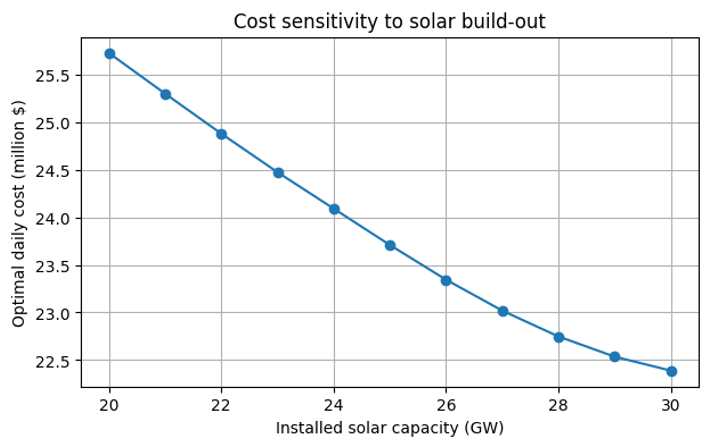
\includegraphics[width=0.8\textwidth]{solar_cost_sensitivity.png}
    \caption{Cost Sensitivity as a function of Installed Solar Capacity from 20 GW (the baseline in 2023) up to 30 GW, a 50\% increase that may be realized in the next decade if V2G is employed.}
    \label{fig:solar_sensitivity}
\end{figure}

Assuming that installed capacity and daily energy generated by solar energy have a linear relationship, we can fit an ARIMA model on solar time series data to forecast how long it will take to increase solar capacity by 50\%. 

\begin{figure}[H]
    \centering
    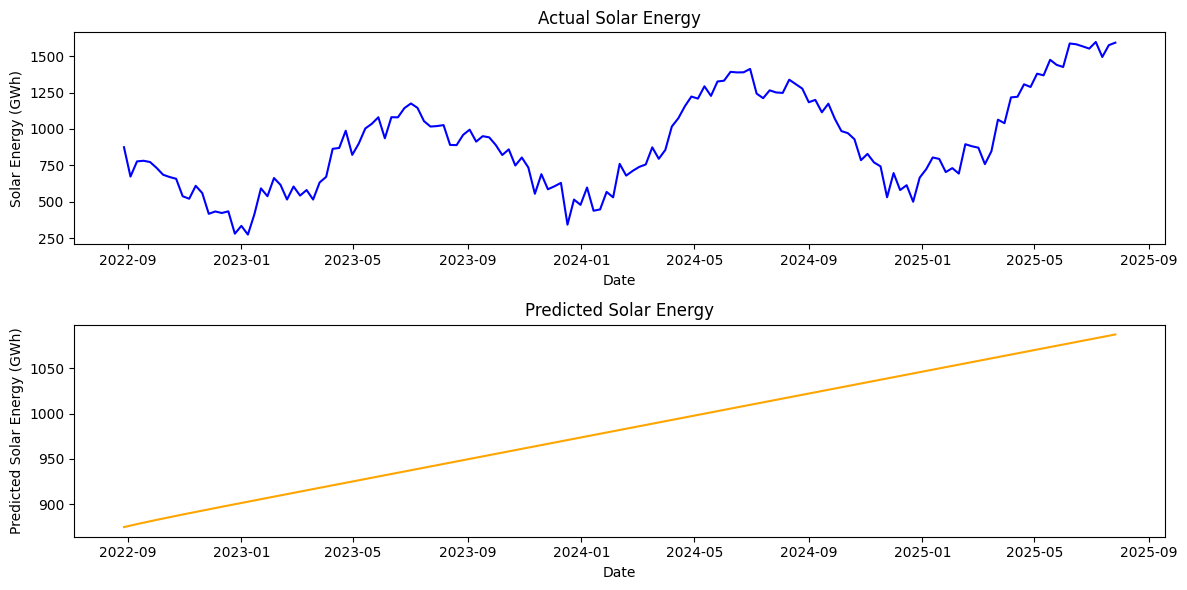
\includegraphics[width=\textwidth]{solar_arima.png}
    \caption{Fitting ARIMA model to solar time-series data}
    \label{fig:solar_arima}
\end{figure}

Although the data show seasonality, the ARIMA algorithm calculates that a model that does not account for seasonality yields the best result, with a MAPE of 37.73. This model predicts that solar capacity will take 391 periods (weeks), starting in August 2025, to increase by 50\%. This translates to approximately 7.5 years. 

\section{Challenges and Opportunities}
While the potential benefits of V2G are substantial, its widespread implementation faces several challenges:
\begin{itemize}
    \item \textbf{Battery Degradation:} Increased charging and discharging cycles can accelerate the degradation of EV batteries, a major concern for vehicle owners. Compensation schemes must be designed to account for this cost.
    \item \textbf{Infrastructure:} Requires the deployment of bidirectional chargers and a sophisticated communication and control network to manage power flow from thousands or millions of vehicles.
    \item \textbf{Consumer Behavior:} The availability of the EV battery bank depends on when and where owners park and plug in their vehicles. Models must account for this variability and uncertainty.
    \item \textbf{Regulatory Framework:} New regulations and market mechanisms are needed to allow EV owners and aggregators to participate in energy markets and be compensated fairly.
\end{itemize}

Despite these hurdles, the opportunities are immense. V2G technology can increase the effective capacity of the grid without building new power plants, support the integration of more renewable energy sources, and provide a new revenue stream for EV owners, thus accelerating the transition to clean transportation and a sustainable energy future.

\section{Summary}
This project demonstrates that leveraging electric vehicle batteries for grid storage is a powerful tool for optimizing utility operations. Our analysis, focused on the California electricity market, reveals that V2G technology can provide substantial daily cost savings by enabling the grid to store cheap renewable energy and redeploy it during peak demand periods. This reduces the reliance on expensive and carbon-intensive peak-generation plants, leading to a cleaner and more affordable energy system. Although significant technical, economic, and regulatory challenges remain, the potential for V2G to help balance the competing demands of cost, reliability, and sustainability makes it a critical area for future research and investment.

Utility companies can use this framework to quantify the potential cost savings and emissions reductions from investing in V2G programs. The model provides a tool for strategic planning, helping to justify infrastructure investments in bidirectional charging and to design incentive programs for EV owners. Future work could extend this deterministic model to a stochastic one, incorporating uncertainty in electricity demand, solar/wind availability, and EV driver behavior. In addition, a sophisticated simulation can be performed to mimic the dynamics of the energy market pricing. Additionally, a more detailed analysis could model battery degradation costs to determine the optimal compensation for EV owners participating in V2G services.

\begin{thebibliography}{9}
\raggedright

\bibitem{1}
Annual CO2 emissions per state from electricity 2023, \url{https://www.eia.gov/environment/emissions/state/}

\bibitem{1}
EIA Levelized Cost of Energy 2023, \url{https://www.eia.gov/outlooks/aeo/electricity_generation/}

\bibitem{1}
State energy demand, \url{https://www.eia.gov/electricity/state/}

\bibitem{1}
EIA Net Generation by type 2023, \url{https://www.eia.gov/electricity/annual/table.php?t=epa_01_01.html}

\bibitem{1}
Battery size capacity, \url{https://www.adamasintel.com/battery-material/ev-battery-capacity-monthly/}

\bibitem{1}
CAISO Daily Generation Capacity, \url{https://www.caiso.com/generation-transmission/generation}

\bibitem{1}
Predictive model of EVs by county, 15.087 Group 5A Final Project SU2025

\end{thebibliography}

\end{document}